\section{Evaluation}
\label{sec:eval}
We build a Java-based tool~\cite{web:githublink} that takes a data schema, a query workload, a number of servers, and an average server memory size and implements our method to automatically produce a data placement configuration.  For now, we require the developer to hand-tune $k$, the number of entity centers, and $m$, the number of pairs of replicated tables and entity groups.  We look to automatically choosing $k$ and $m$ in future work. The results in our experiments use $k=2$ and $m$ as just high enough so that all tables are in a server group.  

\subsection{Benchmark}
\label{sec:benchmark}
We leverage the TPC-H benchmark~\cite{web:tpch} to test the configurations produced by our tool. The benchmark was designed for business applications' query testing purposes. It provides a table schema which has a combination of foreign keys and queries that have varying level of complex joins.

The script \texttt{dbgen} from the TPC-H specification takes in a scaling factor when generating the tables of our choice. By default, it generates all the tables as shown in Figure~\ref{fig:schema}. The scaling factor of 1 generates 1GB dataset which includes all the tables shown in Table~\ref{tab:dataset1gb}.

\comment{
\begin{figure}[!ht]
    \centering
    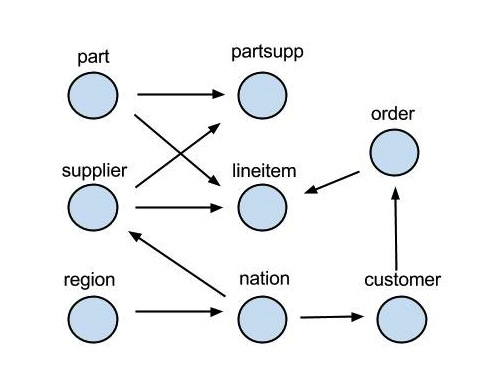
\includegraphics[scale=0.2]{ForeignJoinGraph.jpg}
    \qquad
    \resizebox{3.5cm}{!}{
\begin{tabular}{|c||c|}
\hline
\textbf{Table Name} & \textbf{Number of Rows}\\
\hline
customer & 150 K\\
\hline
lineitem & 6000 K\\ % 6001215
\hline
nation & 25\\
\hline
orders & 1500 K\\
\hline
partsupp & 800 K\\
\hline
part & 200 K\\
\hline
region & 5\\
\hline
supplier & 10 K\\
\hline
\end{tabular}
}
\comment{
    \begin{tabular}[b]{cc}\hline
      Table head & Table head \\ \hline
      Some values & Some values \\
      Some values & Some values \\
      Some values & Some values \\
      Some values & Some values \\
      Some values & Some values \\
      Some values & Some values \\ \hline
    \end{tabular}
    }
    \captionlistentry[table]{A table beside a figure}
    \caption{A table beside a figure}
  \end{figure}
}

\begin{table}
\centering
{%\small
\resizebox{4cm}{!}{
\begin{tabular}{|c||c|}
\hline
\textbf{Table Name} & \textbf{Number of Rows}\\
\hline
customer & 150 K\\
\hline
lineitem & 6000 K\\ % 6001215
\hline
nation & 25\\
\hline
orders & 1500 K\\
\hline
partsupp & 800 K\\
\hline
part & 200 K\\
\hline
region & 5\\
\hline
supplier & 10 K\\
\hline
\end{tabular}
}
}
\caption{\footnotesize{Row distribution for a dataset of size 1 GB.}}
\label{tab:dataset1gb}
\end{table}

The script \texttt{qgen} from the TPC-H specification takes in a query template and generates a query by filling the argument parameters with random values of the corresponding type. For the purpose of this experiment, \texttt{19} of the provided query templates are used, and we create workloads by randomly selecting from the 19 templates and generating 50 queries for each workload.  We create five of such random workloads and evaluate our tool with SQLFire using them.

\comment{
\begin{figure*}[th!]
\centerline{\subfloat[]{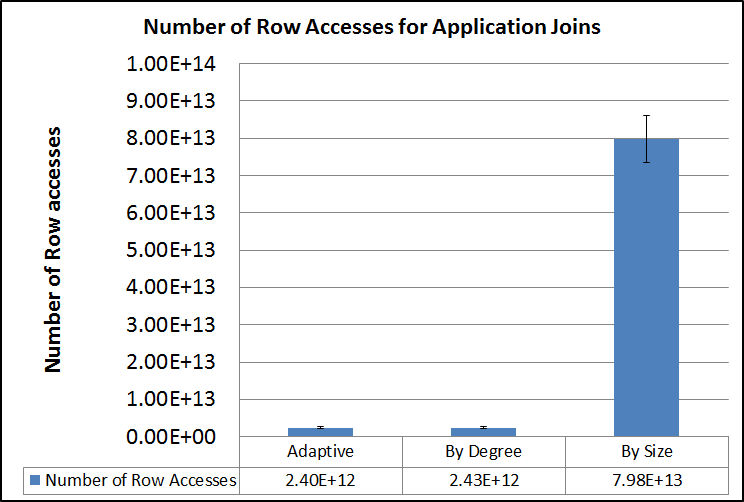
\includegraphics[width=1\columnwidth]{row-accesses.png}
\label{fig:row-accesses}}
\hfil
\subfloat[]{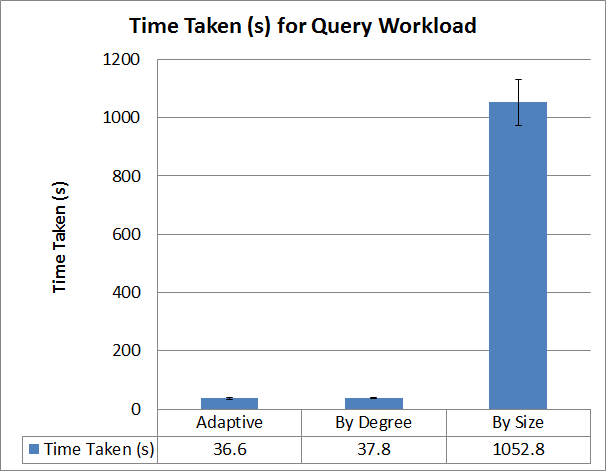
\includegraphics[width=.9\columnwidth]{time-accesses.png}
\label{fig:time-accesses}}}
\caption{\footnotesize{(a) Comparison of the number of row accesses for application-level joins when running the query workload on a dataset of size \texttt{1GB}. (b) Comparison of the time taken when running the query workload on a dataset of size \texttt{1MB}.}}
\label{fig:stats-accesses}
\end{figure*}
}

\subsection{Environment}
\label{sec:environment}
We use four nodes on the Emulab~\cite{web:emulab} network testbed for our system - one node serves as the \texttt{locator} for the SQLFire system which coordinates the data servers.  The remaining three serve as \texttt{data servers} for the tables.  SQLFire keeps the tables in memory, hence we create and populate the tables (with schema Figure~\ref{fig:schema}) with the generated rows whenever the system is restarted. The Emulab nodes have \texttt{64-bit Xeon} processor, \texttt{2 GB} of RAM and are running 64-bit version \texttt{Ubuntu 10.04}.  We, however, only allow data servers to use up to \texttt{0.5 GB} for storing tables.

\begin{figure}
\centering
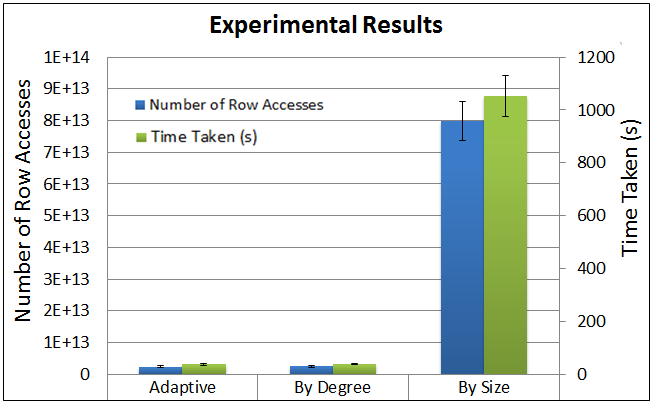
\includegraphics[width=1\columnwidth]{combined-accesses.png}
\caption{\footnotesize{Comparison of the number of row accesses for application-level joins when running the query workload on a dataset of size \texttt{1GB} and time taken to run workload on dataset of size \texttt{1MB}.}}
\label{fig:combined-accesses}
\end{figure}

\subsection{Alternative Placement Strategies}
Alternative viable methods exist for deciding the placement of data in a NewSQL system.  

\begin{itemize}
\vspace*{-9pt}
  \item \emph{Size Strategy} - A method of deciding what tables to partition on, recommended by VMWare in the documentation of SQLFire, is to choose the tables of largest size.  The data of the large tables can then be split evenly amongst the servers of a system.  According to Table \ref{tab:dataset1gb}, this would involve selecting \texttt{lineitem}, \texttt{orders}, and \texttt{partsupp} as entity group "centers" to partition on the primary keys of.  One can then use foreign key relationships to find other tables to partition and colocate with an entity center.  Any tables without foreign key relationships to the entity centers are then chosen to be replicated.
\vspace*{-18pt}
  \item \emph{Degree Strategy} - Another method is to look at the graph of parent to child relationships as in Figure \ref{fig:schema} and choose the tables with the highest degree as entity group centers to partition on the primary keys of.  This would involve selecting \texttt{part}, \texttt{supplier}, and \texttt{nation} to partition on.  One can then partition the children of these tables and colocate them with their parents.  Tables that are not a child of any center are chosen to be replicated.  This strategy is similar to the method we developed except it uses a graph with unweighted edges without consideration of the query workload.
\end{itemize}

\vspace*{-7pt} \noindent While these methods are intuitively sound, our method has the advantage of adapting to query workloads to produce optimized data placement configurations.  We compare our method against the degree and the size strategy in the following sections.
\label{sec:alternative}

\subsection{Experiment}
\label{sec:experiment}
With our experimentation, we aim to quantify and minimize both the number of row accesses performed to execute joins on non-colocated tables in a query workload and the total completion time to execute a query workload.  As of the current release of SQLFire, distributed joins involving tables or partitions that are not colocated on a server are not supported.  In such a case, it is up to the application developer to break a query that uses such joins into table fetches and an application-level join, similar to the case in most NoSQL systems.  

We thus work with this limitation by first modifying TPC-H into a purely join-based workload by stripping all the query templates of any aggregates, sorting, grouping, and non-join filter conditions.  We then write a Java client that uses JDBC to connect to our SQLFire system and sends the queries of our randomly generated TPC-H workloads.  For each query, if we are notified of a failure due to attempting to conduct a distributed join, we separate each join of the failed query into its own separate query.  We then sequentially send the new join queries to the system.  Joins on colocated tables are executed on the data servers, and those that are not colocated are further handled through an application-level join.  Application joins are conducted in a simple manner by fetching both of the tables involved and then having the application scan the entirety of one table for every row in the other table.  We keep track of the number of row accesses that an application needs to do in such application-level joins.  While this is a naive way of performing a join, we use it, as the number of row accesses involved is easily quantified through Equation \ref{eq:cost}.

\subsection{Results}
\label{sec:results}
We use the default TPC-H dataset of size 1GB with our five randomly generated workloads and the data placement configurations produced by our method, the degree strategy, and the size strategy.  The average total number of row accesses for application-level joins in each workload is shown in Figure \ref{fig:combined-accesses} and was calculated using Equation \ref{eq:cost} without actually executing the application joins.  We also measure the time taken to execute the five workloads using the same data placement configurations with executing application-level joins, but with a reduced TPC-H dataset size scaled down to 1MB.  The scaled down dataset size is necessary for our workloads to finish within reasonable amounts of time, as we stripped non-join filter conditions from the queries.  The average number of seconds to complete each workload is also shown in Figure \ref{fig:combined-accesses}.

Interestingly, deciding to partition based on a table's size resulted in a fairly suboptimal configuration for all workloads.  Partitioning based on degree, however, resulted in a configuration that was not much worse than those produced by our adaptive method. We reason that this is due to the random nature of the workload, which causes there to be an equal amount of queries representing each edge of the parent to child join graph, meaning that there is great benefit derived from simply picking nodes with high degree as partition centers.

\subsection{Adaptivity}
\label{sec:adaptivity}
Partitioning based on degree, or any static strategy, is reasonably not a good strategy for handling all kinds of query workloads.  If a query workload happens to place emphasis on a join of tables that are not colocated through the strategy, then it would be fairly detrimental and maladaptive to use the data configuration provided by the strategy.  We test this by generating another TPC-H based workload that will use a query with a join of tables not colocated by the degree strategy 75\% of the time and select from the rest of the queries the remaining 25\% of the time.  We generate 60 queries using this method, and again measure row accesses for application level joins with a \texttt{1GB} dataset and completion time of the entire workload with a \texttt{1MB} dataset.  The results for the workload are shown in Table~\ref{tab:antiDegree}.

As expected, partitioning by degree results in a poor configuration for handling the workload while our method adapts appropriately.  In fact, by focusing 75\% of the workload onto a single join, the size of the set of joins to accommodate for in the workload decreases to the point that our method can colocate all tables involved in joins.

\begin{table}
\centering
\resizebox{6cm}{!}{
    \begin{tabular}{ | c | c | c | p{5cm} |}
        \hline
        \textbf{Strategy} & \textbf{Row Accesses in App. Joins} & \textbf{Time(s)} \\ \hline
        Adaptive & 0.0 &  13\\ \hline
        By Degree & 4.563E13 & 622\\ \hline
        By Size & 1.806E14 & 2674\\
        \hline
    \end{tabular}
    }
\caption{\footnotesize{Results for query workload selected against degree
strategy.}}
\label{tab:antiDegree}
\end{table}

%\begin{figure}
%\centering
%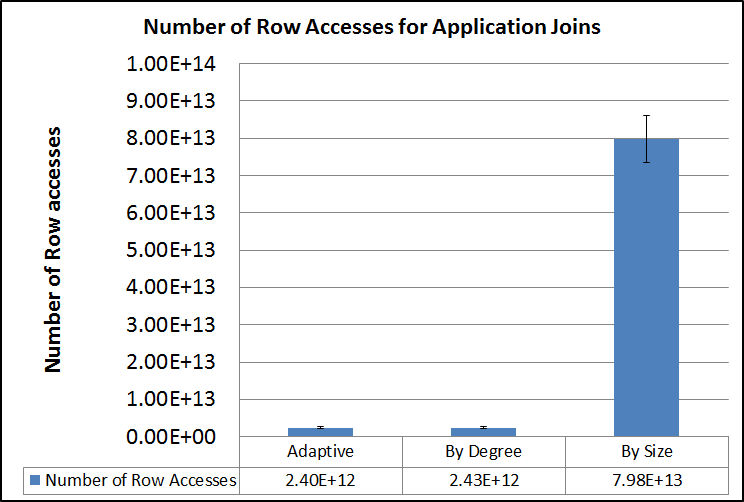
\includegraphics[scale=0.38]{row-accesses.png}
%\caption{Comparison of the number of row accesses for application-level joins when running the query workload on a dataset of size \texttt{1GB}.}
%\label{fig:row-accesses}
%\end{figure}

%\begin{figure}
%\centering
%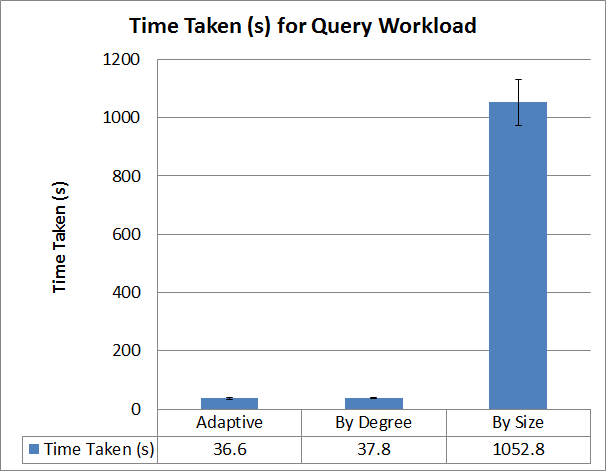
\includegraphics[scale=0.44]{time-accesses.png}
%\caption{Comparison of the time taken when running the query workload on a dataset of size \texttt{1MB}.}
%\label{fig:time-accesses}
%\end{figure}

